\documentclass{beamer}[10]

\usepackage{graphicx}
\usepackage{xcolor}
\usepackage{tabto}
%\usepackage{beamerthemesplit}
\usepackage{tikz}
\usepackage{cancel}
\usepackage{verbatim}
\usepackage{fancybox}
\usepackage{enumerate}
\usepackage{amsmath,amssymb,amsthm,textcomp,mathtools}
\usepackage[super]{nth}
\usepackage[amssymb]{SIunits}
\usepackage{booktabs}
\usepackage{cancel}
\usepackage{bm}
\usepackage[utf8]{inputenc}
\usepackage{tabularx}
\usepackage{ragged2e}
\newcolumntype{Y}{ >{\RaggedRight\arraybackslash}X}
\usetikzlibrary{arrows,shapes}
\newcommand\T{\rule{0pt}{2.6ex}}
\newcommand\B{\rule[-1.2ex]{0pt}{0pt}}
\definecolor{UUcrimson}{RGB}{204,0,0}
\mode<presentation>
{ \usetheme{default}
  \usecolortheme[named=UUcrimson]{structure}
  \useinnertheme{circles}
  \setbeamercovered{transparent}
  \setbeamertemplate{blocks}[rounded]
  \usefonttheme[onlymath]{serif}
  \setbeamertemplate{navigation symbols}{}
  \setbeamertemplate{footline}[page number]
  \setbeamertemplate{navigation symbols}{}
  \setbeamercolor{section in toc}{fg=black,bg=white}
  \setbeamercolor{alerted text}{fg=UUcrimson!80!gray}
  \setbeamercolor*{palette primary}{fg=white,bg=UUcrimson}
  \setbeamercolor*{palette secondary}{fg=UUcrimson!70!black,bg=gray!15!white}
  \setbeamercolor*{palette tertiary}{bg=UUcrimson!80!black,fg=gray!10!white}
  \setbeamercolor*{palette quaternary}{fg=UUcrimson,bg=gray!5!white}
  \setbeamercolor*{palette sidebar primary}{fg=UUcrimson!10!black}
  \setbeamercolor*{palette sidebar secondary}{fg=white}
  \setbeamercolor*{palette sidebar tertiary}{fg=UUcrimson!50!black}
  \setbeamercolor*{palette sidebar quaternary}{fg=gray!10!white}
  \setbeamercolor{titlelike}{parent=palette primary,fg=white}
  \setbeamercolor{frametitle}{bg=UUcrimson}
  \setbeamercolor{frametitle right}{bg=UUcrimson}
  \setbeamercolor*{separation line}{}
  \setbeamercolor*{fine separation line}{}
}

\usetikzlibrary{backgrounds}
\makeatletter
\tikzstyle{every picture}+=[remember picture]
\tikzset{%
  fancy quotes/.style={
    text width=\fq@width pt,
    align=justify,
    inner sep=1em,
    anchor=north west,
    minimum width=\linewidth,
    font=\itshape
  },
  fancy quotes width/.initial={.8\linewidth},
  fancy quotes marks/.style={
    scale=8,
    text=white,
    inner sep=0pt,
  },
  fancy quotes opening/.style={
    fancy quotes marks,
  },
  fancy quotes closing/.style={
    fancy quotes marks,
  },
  fancy quotes background/.style={
    show background rectangle,
    inner frame xsep=0pt,
    background rectangle/.style={
      fill=gray!25,
      rounded corners,
    },
  }
}
\newenvironment{fancyquotes}[1][]{%
\noindent
\tikzpicture[fancy quotes background]
\node[fancy quotes opening,anchor=north west] (fq@ul) at (0,0) {``};
\tikz@scan@one@point\pgfutil@firstofone(fq@ul.east)
\pgfmathsetmacro{\fq@width}{\linewidth - 2*\pgf@x}
\node[fancy quotes,#1] (fq@txt) at (fq@ul.north west) \bgroup}
{\egroup;
\node[overlay,fancy quotes closing,anchor=east] at (fq@txt.south east) {''};
\endtikzpicture}
\makeatother


\usetikzlibrary{backgrounds}
\makeatletter
\tikzstyle{every picture}+=[remember picture]
\tikzset{%
  fancy defs/.style={
    text width=\fq@width pt,
    align=justify,
    inner sep=0.25em,
    anchor=north west,
    minimum width=\linewidth,
    font=\itshape
  },
  fancy defs width/.initial={.8\linewidth},
  fancy defs marks/.style={
    scale=8,
    text=white,
    inner sep=0pt,
  },
  fancy defs opening/.style={
    fancy defs marks,
  },
  fancy defs closing/.style={
    fancy defs marks,
  },
  fancy defs background/.style={
    show background rectangle,
    inner frame xsep=0pt,
    background rectangle/.style={
      fill=gray!25,
      rounded corners,
    },
  }
}
\newenvironment{fancydefs}[1][]{%
\noindent
\tikzpicture[fancy defs background]
\node[fancy defs opening,anchor=north west] (fq@ul) at (0,0) {};
\tikz@scan@one@point\pgfutil@firstofone(fq@ul.east)
\pgfmathsetmacro{\fq@width}{\linewidth - 2*\pgf@x}
\node[fancy defs,#1] (fq@txt) at (fq@ul.north west) \bgroup}
{\egroup;
\node[overlay,fancy defs closing,anchor=east] at (fq@txt.south east) {};
\endtikzpicture}
\makeatother
\usepackage{scalerel}[2014/03/10]
\usepackage{stackengine}
\usepackage{empheq}
\newcommand*\widefbox[1]{\fbox{\hspace{0.5em}#1\hspace{0.5em}}}

\newcommand\reallywidetilde[1]{\ThisStyle{%
  \setbox0=\hbox{$\SavedStyle#1$}%
  \stackengine{-.1\LMpt}{$\SavedStyle#1$}{%
    \stretchto{\scaleto{\SavedStyle\mkern.2mu\sim}{.5467\wd0}}{.4\ht0}%
%    .2mu is the kern imbalance when clipping white space
%    .5467++++ is \ht/[kerned \wd] aspect ratio for \sim glyph
  }{O}{c}{F}{T}{S}%
}}
\usepackage{media9}

\logo{
\includegraphics[width=0.75cm]{logo.jpg}}
\author[Gibbs]{Dr. Jeremy A. Gibbs}
\institute{Department of Mechanical Engineering\\University of Utah}
\date{Spring 2017}
\title{Environmental Fluid Dynamics: Lecture 22}
% colors
\usepackage[loadonly]{enumitem}
\newcommand{\ihat}{\boldsymbol{\hat{\imath}}}
\newcommand{\jhat}{\boldsymbol{\hat{\jmath}}}
\newcommand{\khat}{\boldsymbol{\hat{k}}}
\definecolor{colororange}{HTML}{E65100} % orange
\definecolor{colordgray}{HTML}{795548} % dark gray for note
\definecolor{colorhgray}{HTML}{212121} % heavy dark gray for normal text
\definecolor{colorgreen}{HTML}{009688} % green
\definecolor{colorwhite}{HTML}{FFFFFF} % background white
\definecolor{colorlgray}{HTML}{F5F3EE} % background light gray
\definecolor{colorblue}{HTML}{0277BB} % blue
\definecolor{colorred}{HTML}{CC0000} % red
\newcommand{\fontsizeone}{1.9em}
\usepackage{esvect}
\setbeamertemplate{caption}{\raggedright\insertcaption\par}
\newcommand{\framecard}[2][colorgreen]{
  {\setbeamercolor{background canvas}{bg=#1}
    \begin{frame}[plain]
    \vfill
    \begin{center}
     {#2}
    \end{center}
    \vfill
    \end{frame}
  }
}
\begin{document}

%----------------------------------------------------------------------------------------
%	TITLE & TOC SLIDES
%----------------------------------------------------------------------------------------

\begin{frame} 
  \titlepage
\end{frame}

%------------------------------------------------

\begin{frame}
\frametitle{Overview}
\tableofcontents
\end{frame}

%------------------------------------------------
\section{Integral Forms of Flux-Profile Relationships} %
%------------------------------------------------
\framecard[colorred]{{\color{white}\Huge\begin{center}Integral Forms of~\\Flux-Profile Relationships\end{center}}}
%------------------------------------------------
\subsection{Overview}
%------------------------------------------------
\begin{frame}{Integral Flux-Profile Relationships: Overview}
\begin{itemize}
	\item Dimensionless gradients of velocity, temperature, and moisture are universal functions of $\zeta = z/L$.
	\item We can vertically integrate these gradients to obtain explicit expressions for their profiles.
	\item When this is done, we will build in corrections for static stability.
\end{itemize}
\end{frame}
%------------------------------------------------
\subsection{Momentum}
%------------------------------------------------
\begin{frame}{Integral Flux-Profile Relationships: Momentum}
\begin{itemize}
	\item Integrate flux-profile equation from $z_1$ to $z_2>z_1$ in the ASL
	\begin{align*}
		\frac{\kappa z}{u_*} \frac{\partial \overline{u}}{\partial z} &= \phi_m(\zeta)\\
		\frac{\kappa z}{u_*} \frac{\partial \overline{u}}{\partial z} &= 1 -1 + \phi_m(\zeta)\\
		\frac{\partial \overline{u}}{\partial z} &= \frac{u_*}{\kappa}\left[ \frac{1}{z} - \frac{1-\phi_m(\zeta)}{z}\right]\\
		\int^{z_2}_{z_1} \frac{\partial \overline{u}}{\partial z} dz &= \frac{u_*}{\kappa} \left[ \int^{z_2}_{z_1} \frac{1}{z} dz - \int^{z_2}_{z_1} \frac{1-\phi_m(\zeta)}{z} dz \right]\\
		\overline{u}(z_2) - \overline{u}(z_1) &= \frac{u_*}{\kappa}\left[\ln\left(\frac{z_2}{z_1}\right) - \psi_m\left(\zeta_2, \zeta_1\right)\right]
	\end{align*}
	where $$\psi_m\left(\zeta_2, \zeta_1\right) = \int^{z_2}_{z_1} \frac{1-\phi_m(\zeta)}{z} dz$$
\end{itemize}
\end{frame}
%------------------------------------------------
\begin{frame}{Integral Flux-Profile Relationships: Momentum}
$$\psi_m\left(\zeta_2, \zeta_1\right) = \int^{z_2}_{z_1} \frac{1-\phi_m(\zeta)}{z} dz$$
\begin{itemize}
	\item Let's take $z_1=z_0$ (where $\overline{u}=0$) and $z_2=z>z_0$
	$$\overline{u}(z) = \frac{u_*}{\kappa}\left[\ln\left(\frac{z}{z_0}\right) - \psi_m\left(\zeta, \zeta_0\right)\right]$$
	\item $\psi_m$ is called the \textit{stability correction function} and describes the deviation of the velocity profile from the log-law due to the effect of atmospheric stability.
	\item We generally take $\psi_m(\zeta_0) = 0$ and $\psi_m = \psi_m(\zeta_0)$, which gives the common approximate form
	$$\boxed{\overline{u}(z) = \frac{u_*}{\kappa}\left[\ln\left(\frac{z}{z_0}\right) - \psi_m(\zeta)\right]}$$
\end{itemize}
\end{frame}
%------------------------------------------------
\begin{frame}{Integral Flux-Profile Relationships: Momentum}
\textbf{Stable}
\begin{itemize}
	\item Dyers function
	$$\phi_m(\zeta) = 1 + 5\zeta \quad \text{where } \zeta \geq 0$$
	\item Stability correction function
	\begin{align*}
		\psi_m(\zeta) &= \int^z_0 \frac{1-\phi_m(\zeta)}{z} dz\\
		\psi_m(\zeta) &= \int^z_0 \frac{1-(1+5z/L)}{z} dz\\
		\psi_m(\zeta) &= \int^z_0 -\frac{5}{L} dz = -5\frac{z}{L}\\
		\Aboxed{\psi_h(\zeta) &= -5\zeta}
	\end{align*}
\end{itemize}
\end{frame}
%------------------------------------------------
\begin{frame}{Integral Flux-Profile Relationships: Momentum}
\textbf{Unstable}
\begin{itemize}
	\item Dyers function
	$$\phi_m(\zeta) = (1 - 16\zeta)^{-1/4}  \quad \text{where } \zeta \leq 0$$
	\item Stability correction function
	~\\~\\Apply a similar procedure and use a standard integral table to arrive at
	\begin{empheq}[box=\widefbox]{align*}
		&\psi_m(\zeta) = 2\ln\left(\frac{1+x}{2}\right) + \ln\left(\frac{1+x^2}{2}\right) - 2\tan^{-1}x + \frac{\pi}{2}\\\\
		&\text{where } x = \phi_m^{-1} = (1 - 16\zeta)^{1/4}
	\end{empheq}
\end{itemize}
\end{frame}
%------------------------------------------------
\begin{frame}{Integral Flux-Profile Relationships: Momentum}
\begin{figure}
	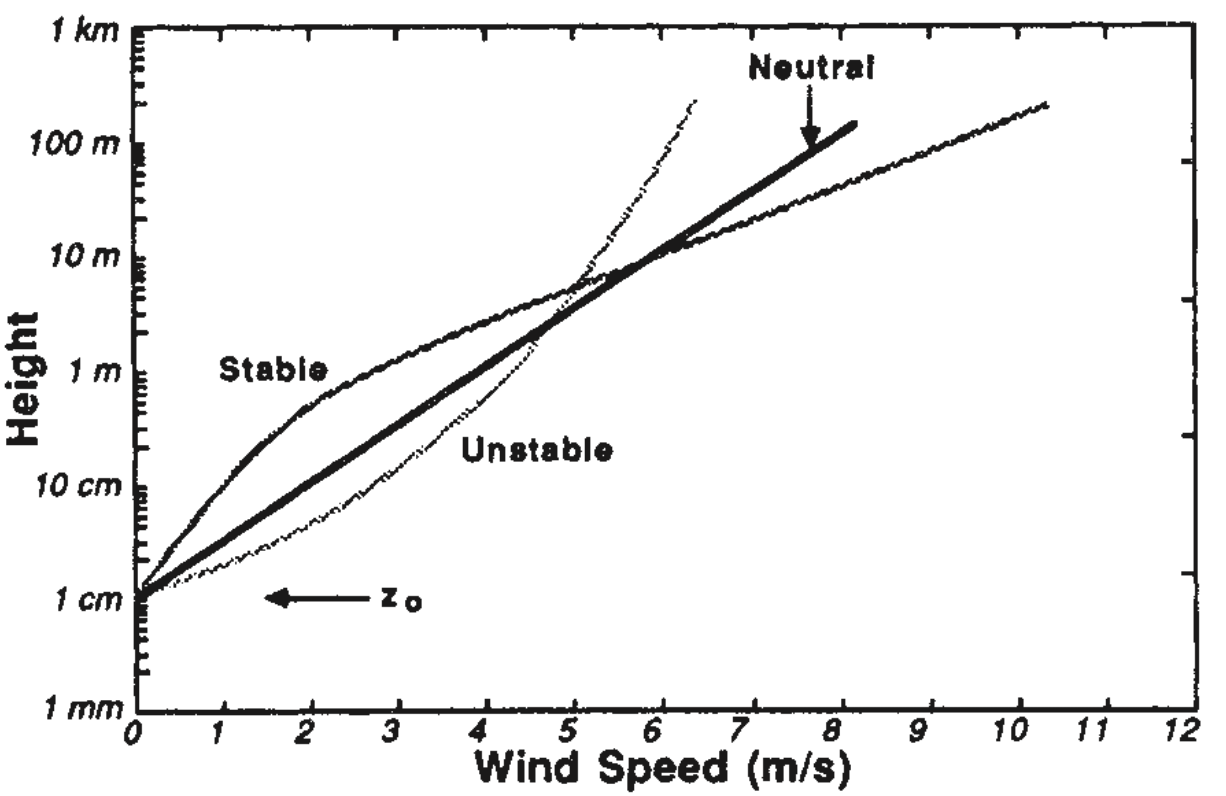
\includegraphics[width=\textwidth]{loglaw1}
\end{figure}
\centering \tiny Fig 9.5 from Stull (1988)
\end{frame}
%------------------------------------------------
\begin{frame}{Integral Flux-Profile Relationships: Momentum}
\begin{figure}
	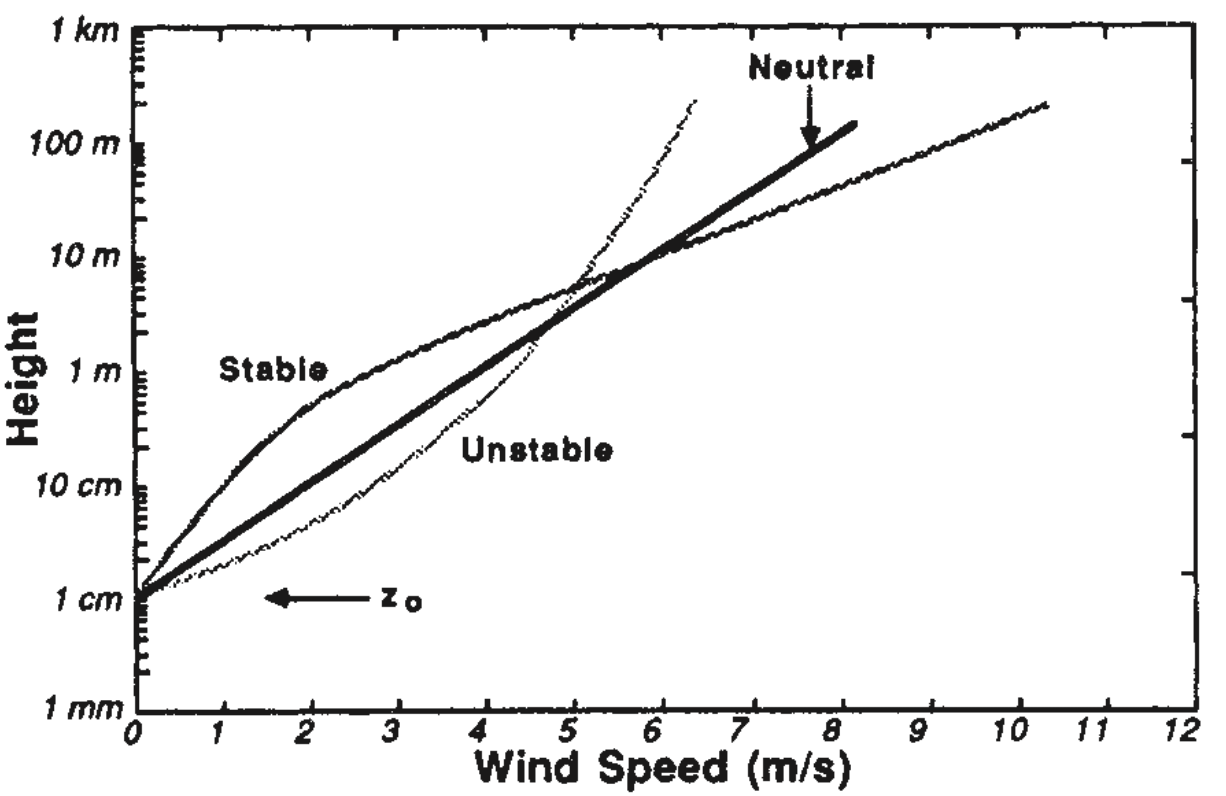
\includegraphics[width=0.5\textwidth]{loglaw1}
\end{figure}
\begin{itemize}
	\item Deviations from the log-law increase with increasing $|\zeta|$
	\item Under stable conditions, the profiles are log-linear and tend to become linear for large $\zeta$.
	\item For unstable conditions, $\psi_m, \psi_h > 0$, so deviations are negative. Accordingly, the profiles become increasingly curvilinear for large $|\zeta|$. 
\end{itemize}
\end{frame}
%------------------------------------------------
\subsection{Heat/Moisture}
%------------------------------------------------
\begin{frame}{Integral Flux-Profile Relationships: Heat/Moisture}
\begin{itemize}
	\item Integrate flux-profile equation from $z_1$ to $z_2>z_1$ in the ASL
	\begin{align*}
		\frac{\kappa z}{\theta_*} \frac{\partial \overline{\theta}}{\partial z} &= \phi_h(\zeta)\\
		\frac{\kappa z}{\theta_*} \frac{\partial \overline{\theta}}{\partial z} &= 1 -1 + \phi_h(\zeta)\\
		\frac{\partial \overline{\theta}}{\partial z} &= \frac{\theta_*}{\kappa}\left[ \frac{1}{z} - \frac{1-\phi_h(\zeta)}{z}\right]\\
		\int^{z_2}_{z_1} \frac{\partial \overline{\theta}}{\partial z} dz &= \frac{\theta_*}{\kappa} \left[ \int^{z_2}_{z_1} \frac{1}{z} dz - \int^{z_2}_{z_1} \frac{1-\phi_h(\zeta)}{z} dz \right]\\
		\overline{\theta}(z_2) - \overline{\theta}(z_1) &= \frac{\theta_*}{\kappa}\left[\ln\left(\frac{z_2}{z_1}\right) - \psi_h\left(\zeta_2, \zeta_1\right)\right]
	\end{align*}
	where $$\psi_h\left(\zeta_2, \zeta_1\right) = \int^{z_2}_{z_1} \frac{1-\phi_h(\zeta)}{z} dz$$
\end{itemize}
\end{frame}
%------------------------------------------------
\begin{frame}{Integral Flux-Profile Relationships: Heat/Moisture}
$$\psi_h\left(\zeta_2, \zeta_1\right) = \int^{z_2}_{z_1} \frac{1-\phi_h(\zeta)}{z} dz$$
\begin{itemize}
	\item Let's take $z_1=z_{0\theta}$ (where $\overline{\theta}=\theta_s$) and $z_2=z>z_{0\theta}$
	$$\overline{\theta}(z) = \theta_s + \frac{\theta_*}{\kappa}\left[\ln\left(\frac{z}{z_{0\theta}}\right) - \psi_h\left(\zeta, \zeta_0\right)\right]$$
	\item Take $\psi_h(\zeta_{0\theta}) = 0$ and $\psi_h = \psi_h(\zeta_{0\theta})$, which gives the common approximate form
	$$\boxed{\overline{\theta}(z) = \theta_s + \frac{\theta_*}{\kappa}\left[\ln\left(\frac{z}{z_{0\theta}}\right) - \psi_h(\zeta)\right]}$$
	\item Similarly,
	$$\boxed{\overline{q}(z) = q_s + \frac{q_*}{\kappa}\left[\ln\left(\frac{z}{z_{0q}}\right) - \psi_h(\zeta)\right]}$$
\end{itemize}
\end{frame}
%------------------------------------------------
\begin{frame}{Integral Flux-Profile Relationships: Heat/Moisture}
\textbf{Stable}
\begin{itemize}
	\item Dyers function
	$$\phi_h(\zeta) = 1 + 5\zeta \quad \text{where } \zeta \geq 0$$
	\item Stability correction function
	\begin{align*}
		\psi_h(\zeta) &= \int^z_0 \frac{1-\phi_h(\zeta)}{z} dz\\
		\psi_h(\zeta) &= \int^z_0 \frac{1-(1+5z/L)}{z} dz\\
		\psi_h(\zeta) &= \int^z_0 -\frac{5}{L} dz = -5\frac{z}{L}\\
		\Aboxed{\psi_m(\zeta) &= -5\zeta}
	\end{align*}
\end{itemize}
\end{frame}
%------------------------------------------------
\begin{frame}{Integral Flux-Profile Relationships: Heat/Moisture}
\textbf{Unstable}
\begin{itemize}
	\item Dyers function
	$$\phi_h(\zeta) = (1 - 16\zeta)^{-1/2}  \quad \text{where } \zeta \leq 0$$
	\item Stability correction function
	~\\~\\Apply a similar procedure and use a standard integral table to arrive at
	\begin{empheq}[box=\widefbox]{align*}
		&\psi_h(\zeta) = 2\ln\left(\frac{1+y}{2}\right)\\\\
		&\text{where } y = \phi_h^{-1} = (1 - 16\zeta)^{1/2}
	\end{empheq}
\end{itemize}
\end{frame}
%------------------------------------------------
\subsection{Calculation of Surface Turbulent Fluxes}
%------------------------------------------------
\begin{frame}{Calculation of Surface Turbulent Fluxes}
\begin{itemize}
	\item Here is a practical guide for how to compute surface turbulent fluxes in the case of non-coinciding measurements/model levels.
	\item In this scenario, we have mean values of $u$,$T(\text{abs. temp})$, and $q$ measured at $u_1, u_2$ at $z_{u1}, z_{u2}$, $T_1 \approx \theta_1, T_2\approx \theta_2$ at $z_{\theta 1}, z_{\theta 2}$, and $q_1, q_2$ at $z_{q1}, z_{q2}$. 
	\item $p$ is known at one of measurement level and $\beta$ and $\rho$ can also be evaluated.
\end{itemize}
\end{frame}
%------------------------------------------------
\begin{frame}{Calculation of Surface Turbulent Fluxes}
\begin{enumerate}
	\item First approximation: $u$, $\theta$, and $q$ are neutral and logarithmic
	\begin{align*}
	u_2 - u_1 &= \frac{u_*}{\kappa} \ln\frac{z_{u2}}{z_{u1}}\\
	\theta_2 - \theta_1 &= \frac{\theta_*}{\kappa} \ln\frac{z_{\theta 2}}{z_{\theta 1}}\\
	q_2 - q_1 &= \frac{q_*}{\kappa} \ln\frac{z_{q2}}{z_{q1}}
	\end{align*}
	which gives a first guess of the turbulence scales
	\begin{align*}
	u_* = \frac{\kappa(u_2 - u_1)}{\ln (z_{u2}/z_{u1})}\\
	\theta_* = \frac{\kappa(\theta_2 - \theta_1)}{\ln (z_{\theta 2}/z_{\theta 1})}\\
	q_* = \frac{\kappa(q_2 - q_1)}{\ln (z_{q2}/z_{q1})}
	\end{align*}
\end{enumerate}
\end{frame}
%------------------------------------------------
\begin{frame}{Calculation of Surface Turbulent Fluxes}
\begin{enumerate}
\setcounter{enumi}{1}
	\item Based on those scales, evaluate the Obukhov length
	$$L = \frac{u_*^2}{\kappa(\beta \theta_* + 0.61 g q_*)}$$
	\item If $z_h/|L|\ll 1$ ($z_h$ = highest measurement level), the flow is considered neutral. It is reasonable to take $z_h/|L|=0.01$ as the lower limit for the non-neutral case. ~\\~\\In a near-neutral ASL ($z_h/|L|<0.01$), kinematic fluxes are evaluated based on the computed scales.
	\begin{align*}
		\overline{w^\prime u^\prime} &= -u_*^2\\
		\overline{w^\prime \theta^\prime} &= -u_*\theta_*\\
		\overline{w^\prime q^\prime} &= -u_*q*
	\end{align*}
\end{enumerate}
\end{frame}
%------------------------------------------------
\begin{frame}{Calculation of Surface Turbulent Fluxes}
\begin{enumerate}
\setcounter{enumi}{3}
	\item \label{itm:four} If $z_h/|L|\geq 0.01$, we proceed to new approximations of the turbulence scales
	\begin{align*}
		u_* = \frac{\kappa(u_2 - u_1)}{\left[\ln \left(\cfrac{z_{u2}}{z_{u1}}\right) - \psi_m(\zeta_{u2}) + \psi_m(\zeta_{u1})\right]}\\
		\theta_* = \frac{\kappa(\theta_2 - \theta_1)}{\left[\ln \left(\cfrac{z_{\theta 2}}{z_{\theta 1}}\right) - \psi_h(\zeta_{\theta 2}) + \psi_h(\zeta_{\theta 1})\right]}\\
		q_* = \frac{\kappa(q_2 - q_1)}{\left[\ln \left(\cfrac{z_{q2}}{z_{q1}}\right) - \psi_h(\zeta_{q2}) + \psi_h(\zeta_{q1})\right]}\\
	\end{align*}
	making sure to account for the sign of $L$ and applying the proper stability correction functions.
\end{enumerate}
\end{frame}
%------------------------------------------------
\begin{frame}{Calculation of Surface Turbulent Fluxes}
\begin{enumerate}
\setcounter{enumi}{4}
	\item \label{itm:five} Based on the new scales, evaluate the Obukhov length
	$$L = \frac{u_*^2}{\kappa(\beta \theta_* + 0.61 g q_*)}$$
	\item Steps \ref{itm:four} and \ref{itm:five} are repeated until the difference between the new and old values of $L$ reach a minimum threshold ($\sim 0.01$).
	\item Based on computed scales, compute kinematic fluxes as
	\begin{align*}
		\overline{w^\prime u^\prime} &= -u_*^2\\
		\overline{w^\prime \theta^\prime} &= -u_*\theta_*\\
		\overline{w^\prime q^\prime} &= -u_*q*
	\end{align*}
\end{enumerate}
\end{frame}
%------------------------------------------------
\begin{frame}{Calculation of Surface Turbulent Fluxes}
\begin{enumerate}
\setcounter{enumi}{7}
	\item Finally, $u$, $\theta$, and $q$ are obtained at any level $z$ in the ASL:
	\begin{align*}
	u(z) &= u_1+ \frac{u_*}{\kappa}\left[\ln \left(\cfrac{z}{z_{u1}}\right) - \psi_m(\zeta) + \psi_m(\zeta_{u1})\right]\\
	\theta(z) &= \theta_1+ \frac{\theta_*}{\kappa}\left[\ln \left(\cfrac{z}{z_{\theta 1}}\right) - \psi_h(\zeta) + \psi_h(\zeta_{\theta 1})\right]\\
	q(z) &= q_1+ \frac{q_*}{\kappa}\left[\ln \left(\cfrac{z}{z_{q1}}\right) - \psi_h(\zeta) + \psi_h(\zeta_{q1})\right]	
	\end{align*}
	Note: In this case, $z>z_{u1},z_{\theta 1},z_{q1}$. However, you can use values of $u$, $\theta$, and $q$ at some height $z_{u2},z_{\theta 2},z_{q2}$ to obtain their respective values at some height $z<z_{u2},z_{\theta 2},z_{q2}$
\end{enumerate}
\end{frame}
%------------------------------------------------
\end{document}

